\newpage
\section{Opgavebesvarelse}\label{sec:OpgaveBesvarelse}

\subsection{Fra Hemmelige Øjne til de digitale Skygger}\label{sec:Redegorsel}
For at få en godt forståelse skal tiden spoles tilbage til 500 år f.v.t. Her skrev den kinesiske strateg og hærfører Sun Tsu om vigtigheden af at bruge agenter og dobbeltagenter. Når et land eller en hærfører havde agenter kunne han/hun vinde nemmere angreb,  det kom desuden også men en fordel om at de kunne komme angrebene i forkøbet. \\ Sun Tsu sagde: \emph{"One who knows the enemy and knows himself will not be endangered in a hundred engagements."} Værket hedder "13 afsnit om militærstrategi" og er i dag en af de mest populære bøger om strategi. Værket lægger vægt på de politiske hensyn i krigsførelse og er understøttet af filosofiske og metafysiske overvejelser. (\cite{SunTsu})
Efter Sun Tsu's tid har spionage ændret sig en del, og der er sket en markant forandring. Den tid der for opgaven her er mest interesseret, er dog tiden omkring Den Kolde Krig. Under Den Kolde Krig var spionage ikke blot en sprøgsmål om militær efterretning, men en central del af den ideologiske og politiske kamp mellem Øst og Vest. Den østtyske sikkerhedstjenste, Stasi  anno 1949-1990 (Ministerium für Staatsicherheit) var en af de nok mest effektive og frygtende efterretningstjenester i verden. Stasi havede en bred og ommenfattende overvånings strategi. Hvor man både tillod at aflytte befolkningen, men også udlandske personer såsom diplomater. Stasi's arbejde involverede ikke kun traditionel spionage som skygning, muldvarper, og sexspionage. (\cite{stasi}) De anvendte også mere avanceret udstyr til at overvåge. Dette var blandet andet overvåning af FM kanaler, mv. Under Stasi's tid begynder udruldningen af aflytningsudstyr for alvor. Man kan nu gemme mikrofoner i vægge, lamper, og meget andet. Deres arbejde var omfattende og man havde derfor en stor mængde af agenter. Man anslår at der var 1 Stasi agent for hver 166 østtysker. Dette er en meget stor mængde. Altså var der cirka 90.000 Stasi agenter i østtyskland. Mange af dem var enten friviligt eller under tvang. Stasi's indflydelse strakte sig langt ud over DDR's grænser. En af de mest bemærkelsesværdige operationer var infiltreringen af Vesttyskland. Et godt og konkret eksempel på netop dette var Stasi's arbejde under en operation der omhandlde den vesttyske agent Günter Guillaume. Operationen kendes også under navnet Gulliamen affæren. Günter Guillaume arbejdede som rådgiver for Vesttysklands kansler Willy Brandt. Guillaume var en hemmelig Stasi-agent, der i mange år leverede følsomme oplysninger til Østtyskland. Hans afsløring i 1974 førte til en stor skandale og tvang Willy Brandt til at træde tilbage som kansler. Denne episode demonstrerer Stasi's evne til at infiltrere højtstående politiske kredse og påvirke den vesttyske regering. (\cite{guillaume})

\subsubsection{Hvad med det der privatliv?} % Skriv konkret om John Locke og hans tanker om privatlivets fred
Privatlivets fred er en grundlæggende menneskerettighed, der omfatter individets ret til at leve sit eget liv uden unødvendig indblanding fra staten, andre borgere eller private organisationer. Det indebærer beskyttelse af personlige oplysninger, kommunikation og ejendom samt retten til at træffe personlige beslutninger uden at blive overvåget eller kontrolleret. Denne rettighed er afgørende for individets frihed og værdighed. Den er beskyttet af internationale menneskerettighedskonventioner, såsom FN's Verdenserklæring om Menneskerettigheder og Den Europæiske Menneskerettighedskonvention. (\cite{LockeFaktalink})
John Locke, en af de mest indflydelsesrige filosoffer i oplysningstiden, bidrog væsenligt til at definere forståelsen af privatlivets fred. Locke definerede privatlivets fred i gennem sine værker. Locke argumentede for at mennesker i dens natur er klog nok til at kunne træffe beslutninger for sig selv, og at man derfor måtte lade mennesket værne om sig selv. Han definerede grundlæggende rettigheder så som retten til livet, frihed, og ejendom. Locke definerede desuden at dette ikke var rettigheder en fyrste eller et demokrati udstedet men at det var medfødte rettigheder som alle mennesker har. (\cite{LockeFaktalink})
I sit værk "Two Treatises og Goverment" (1689) definerer Locke privatlivets fred som en del af retten til ejendom. For Locke omfatter ejendom ikke kun matrielle gendstande, men også ens person, handlinger og ideer. Han mente, at individets frihed og ejendom slulle beskyttes mod vilkårlig indblanding fra staten, eller andre individer. Ifølge Locke er formålet med regeringen at beskytte disse rettigheder, og hvis en regering ikke beskytter disse eller krænker dem, er det en hvermands ret at vælte regeringen. Lockes filosofi understreger vigtigheden af en begrænset regering, der respekterer individets rettigheder, og handler inden for lovens fire rammer. Han mente, at love skulle baseres på samtykke fra de valgte/regede og skulle tjene til at beskytte deres naturlige rettigheder. Dette princip er grundlaget for moderne liberale demokratier og deres respekt for privatlivets fred. (\cite{LockeBog})
I den danske grundlov er retten til privatlivet beskyttet, og det er ulovligt for regeringen at indsamle oplysninger om borgerne uden samtykke eller en dommerkendelse. Desuden er retten til ejendom også beskyttet, dette er nedfæsteret som den private ejendomsret. \\\\ \emph{"§ 73. Stk. 1. Ejendomsretten er ukrænkelig. Ingen kan tilpligtes at afstå sin ejendom, uden hvor almenvellet kræver det. Det kan kun ske ifølge lov og mod fuldstændig erstatning."} \\ \\
Privatlivets fred, som Locke definerede det, har direkte relevans for spørgsmålet om statslig spionage og overvågning. Efterretningstjenesters overvågningsaktiviteter kan udgøre en trussel mod individets rettigheder, hvis de ikke udføres inden for rammerne af loven og med passende tilsyn. Balancen mellem national sikkerhed og beskyttelsen af borgernes privatliv er en kompleks udfordring, der kræver omhyggelig afvejning af behovet for sikkerhed og respekten for individuelle frihedsrettigheder. Lockes tanker om privatlivets fred understreger, at selvom regeringen har en legitim interesse i at beskytte nationens sikkerhed, må dette ikke ske på bekostning af individets grundlæggende rettigheder. Enhver form for overvågning skal derfor være nødvendigheds- og proportionalitetsafprøvet, og der skal være mekanismer på plads for at sikre, at borgernes rettigheder respekteres og beskyttes.

\newpage
\subsection{Spywere program}
Der er blevet programeret et spywere program med forskellige funktioner. Programmet er skrevet og udviklet i sproget python, i opgaven er der anvendt funktionel programmering til at skrive programmet. Grunden til at der er anvende funktionel programmering er at det vil være den smarteste løsning. Hvis objektorientering anvendes vil man støde ind i det problem at når programmet bliver udløst så vil det give et drop i hvor hurtigt computeren er. 80 årige Bente vil måske ikke opdage det, men professionelle spioner og data analytikere, vil lyn hurtigt opdage at der hver 10 sekund bliver oprettet en ny instans af programmet. Dette vil dog ikke ske i samme grad når der anvendes funktionel programmering. Her vil instansen nemlig stadig være aktiv. Og derfor vil ikke de omfattede personer ikke opdage at programmet direkte bliver udløst mens man anvender programmet. Programmet er cirka lige så godt som cæsar kryptering er på computerer nu tildags. Med andre ord det er slet ikke godt, og man kan ikke bruge det til noget efterretningsarbejde. Programmet er dog stadig et godt eksempel på hvordan og hvad form for data der indsamles. Følgende data indsmales i programmet her: Screenshot, og webcam. Programmet er skrevet således at det tager et screenshot og et billede af dit webcam hvert 10 sekund. Programmet er skrevet således at det gemmer dataen i en fil. Og der skal derfor ikke skrives ret meget mere kode for at den bare kan sende dataen til en server.
\begin{figure}[h!]
    \centering
    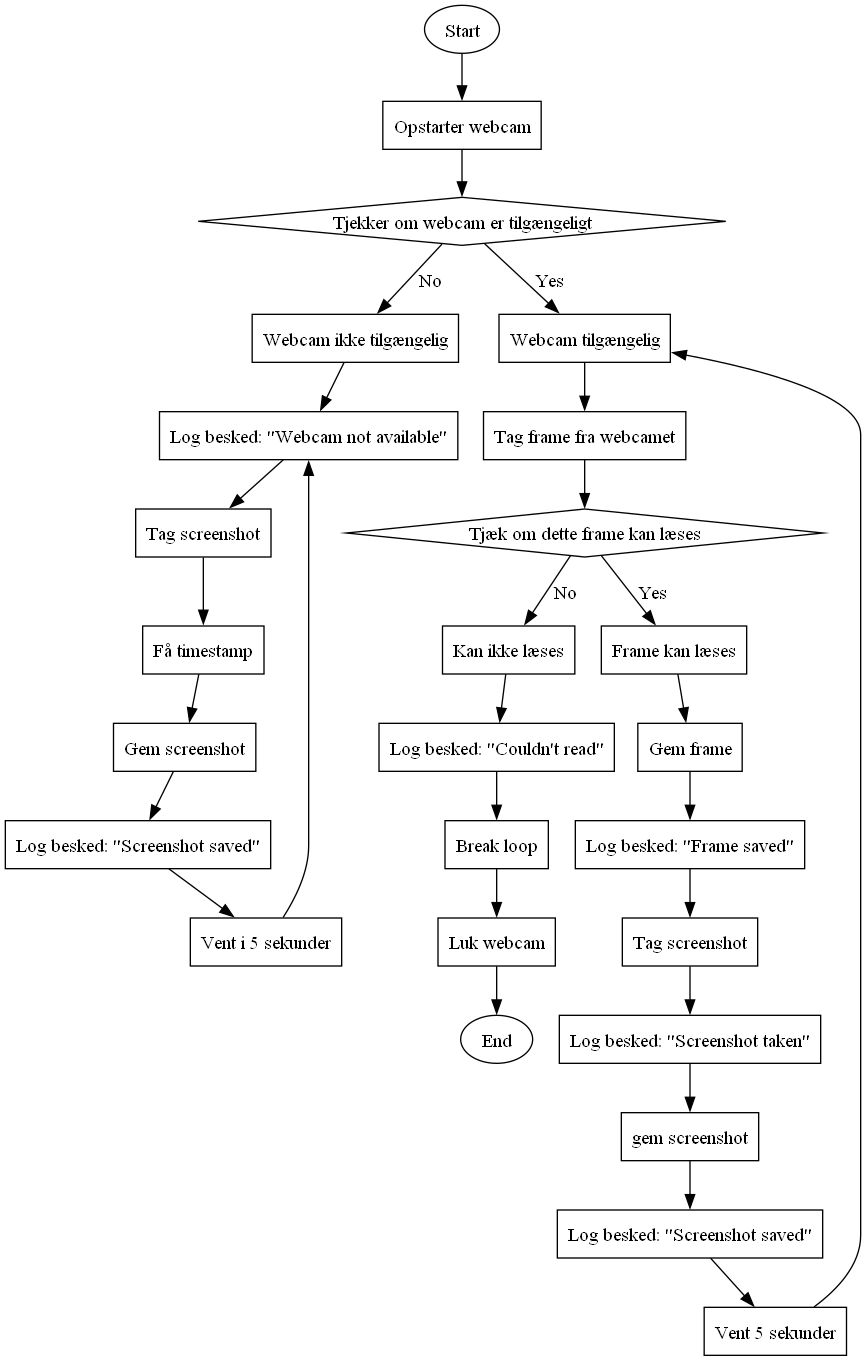
\includegraphics[width=0.5\textwidth]{figurs/flow.png}
    \caption{Spywere program flowchart}
    \label{fig:Spywere}
\end{figure}
\\ Der bliver i koden anvendt en række forskellige biblioteker. Disse biblioteker er: Tid, CV2, pyautogui og pillow. Under ideelle omstændiger ville man ej heller anvende disse biblioteker. Dette skydes mange forskellige ting. En af de ting som klart gør at man ikke vil anvende sådan noget som OpenCV er fordi den sprøger computeren om den må anvende kammeraet. Dette ønsker man ikke når man gerne vil være skjult. Desuden er ulempen ved at bruge disse biblioteker at man nemt lige kan lave et program der kan opdage disse biblioteker. Og man bliver derfor hurtigt opdaget. For at give en bedre forståelse for koden, vil der nu blive givet en ganske kort gennemgang/analyse af koden.
\begin{python}
    cap = cv2.VideoCapture(0)
\end{python}
Denne linje kode er nok den vigtigste linje for at kammeraet fungere. Dette er nemlig den linje hvorfor man inzialisere kammeraet. Her går man efter kammeraet med indexet 0. Køres denne linje ikke vil selve kamera delen ikke fungere. 
\begin{python}
    if not cap.isOpened(): # Check if the webcam is opened correctly
        print("Webcam not available")
        while True:
            screenshot = pyautogui.screenshot() # Take a screenshot
            timestamp = time.strftime("%Y%m%d-%H%M%S") # Get the current time
            filename = f"screenshot_{timestamp}.png" # Define the filename
            screenshot.save(filename) # Save the screenshot
            print(f"Screenshot saved as {filename}")
            time.sleep(5) # Wait 5 seconds before taking a new screenshot
\end{python}
Programmet spørger her om det kan finde kammeraet. Hvis det ikke kan det vil programmet kun tage et screenshot. Kan den tilgå kammeraet så vil programmet fortsætter til den else statment der er længere nede i koden. Dette vil programmet gøre hvert 5 sekund. I programmet er der ikke lavet en failsafe som tjekker hvert 10 sekundt som lige tjekker op på om det nu kan tilgå kammeraet. Programmet tjekker en gang og det er når programmet køres første gang. Når dette er tjekket af vil programmet gå videre til at tage billeder af skærmen. Dette sker ved at et while loop aktiveres. Dette while loop køre i \begin{math}O^n\end{math} og stopper derfor aldrig. Først ber python programmet om at tage et screenshot. Herefter ber programmet tids modulet om hvad tiden er, herefter defineres filnavnet. Efter dette gemmes filen under det fil navn der er generet. Et eksempel på et fil navn kunne være screenshot\_2020122411112.png for lige at dele det op, så er det første ord $screenshot$ dette definere hvad type data, efter det kommer tiden $20201224$ dette er datoen. (Y, M. D) og til sidst kommer tiden $11112$ dette er hvad klokken var lige i det skærmbilledet blev taget. (H, M, S) Programmet vil gemme filen i samme mappe som programmet ligger i. Programmet vil herefter Logge at filen er gemt. Tilsidst vil programmet vente i 5 sekundt og så tage et nyt screenshot. 
\begin{python}
    else:
        while True:
            ret, frame = cap.read()
            if not ret:
                print("Couldn't read")
                break
            timestamp = time.strftime("%Y%m%d-%H%M%S")
            filename = f"image_{timestamp}.jpg"
            cv2.imwrite(filename, frame)
            print(f"Frame saved as {filename}")

            print("Taking screenshot")
            screenshot = pyautogui.screenshot()
            print("Screenshot taken")
            timestamp = time.strftime("%Y%m%d-%H%M%S")
            filenameScreenShot = f"screenshot_{timestamp}.png"

            screenshot.save(filenameScreenShot)
            print(f"Screenshot saved as {filenameScreenShot}")
            time.sleep(5)
\end{python}
Denne del af koden aktiveres hvis kammeraet er aktiveret og at programmet kan tilgå den. Der vil her ikke blive beskrevet hvordan screenshot delen virker da dette allrede er beskrevet. Først forsøger programmet at læse en remme fra webcam'et \pythoninline{ret, frame = cap.read()} Hvis læsningen lykkes (ret er True), gemmes billeddataene i frame. Hvis læsningen fejler (ret er False), udskrives en fejlmeddelelse, og løkken brydes med break. Ellers fungere det meget ligesom screenshot delen. Programmer ber cv2 om at gemme framet. Billedet/framet for et navn baseret på dato og tid også gemmes det. Til sidst ventes der i 5 sekundter og så tages der et nyt billede. Dette Python program er et effektivt værktøj til at kontinuerligt lave billedoptagelse fra et webcam og tage screenshots. Programmet kombinerer brugen af flere biblioteker - OpenCV til webcam interaktion, PyAutoGUI til skærmoptagelser, og Pillow til billedlagring - hvilket gør det alsidigt og kraftfuldt.

\subsection{Hvordan skal man forholde sig til spionage?}
Spionage er en kompleks og kontroversiel praksis, der rejser en række etiske og juridiske problemstillinger. Når spionage og spyware skal vurderes, er det vigtigt at overveje de potentielle konsekvenser for individets rettigheder og friheder. Inddrages Aristoteles i denne vurdering, kunne han argumentere for, at retfærdighed opnås gennem en balance mellem individets rettigheder og samfundets interesser. På den ene side kan spionage være et effektivt og nødvendigt redskab til at beskytte nationen. På den anden side udgør det imidlertid også et klart brud på privatlivets fred og kan krænke individets naturlige rettigheder. \\John Locke argumenterede for, at regeringen har pligt til at beskytte individets rettigheder, herunder retten til liv, frihed og ejendom. Enhver form for statslig overvågning eller indgriben i individets privatliv bør derfor, ifølge både Aristoteles og Locke, kun ske, hvor det er absolut nødvendigt. Det er derfor afgørende at finde den af Aristoteles beskrevne middelvej. At finde balancen mellem behovet for sikkerhed og respekten for de naturlige rettigheder beskrevet af Locke kan volde store problemer. \\ Dette kræver, at statslige efterretningsorganisationer overholder lovgivningens rammer. De skal respektere individets rettigheder og udvise gennemsigtighed og ansvarlighed i deres handlinger. Der skal være passende kontrolmekanismer på plads for at sikre, at spionageaktiviteter udføres på en retfærdig og lovlig måde og ikke misbruges til politiske eller personlige formål. Der skal anvendes et proportionalitetsprincip, hvor omfanget af overvågning skal stå i rimeligt forhold til den formodede trussel eller forbrydelse. For eksempel bør en simpel lommetyv ikke totalovervåges med spyware, mikrofoner og kameraer.\\ Det er ikke altid muligt at finde den perfekte balance mellem sikkerhed og privatlivets fred. Der vil være situationer, hvor der trædes forkert, og netop her er det vigtigt, at der er kontrolmekanismer på plads, som kan gribe ind tidligt. Det er derfor også vigtigt, at magtens tredeling fungerer effektivt, således at en kontrolinstans kan stoppe misbrug af magt, før det løber løbsk.

\subsubsection{Vigtigheden af Privatlivets Fred i et Demokratisk Samfund}
I et demokratisk samfund er privatlivets fred en af de mest grundlæggende rettigheder, der beskytter borgerne mod vilkårlig indblanding fra staten. Privatlivets fred sikrer, at individer kan tænke, kommunikere og handle uden ubegrundet frygt for overvågning. Denne frihed er essentiel for individets muligheder for at udøve andre grundlæggende rettigheder, såsom ytrings-, religions- og forsamlingsfrihed. John Locke understregede, at en regerings legitimitet hviler på dens evne til at beskytte individets naturlige rettigheder, herunder retten til privatliv. Uden denne beskyttelse kan borgerne miste tilliden til staten, hvilket undergraver demokratiets fundament. Locke mente, at når staten krænker disse rettigheder, bliver det borgernes ret og pligt at modsætte sig og søge retfærdighed. Aristoteles' filosofi om retfærdighed og balance er også relevant her. Han ville argumentere for, at retfærdighed indebærer, at individet får den beskyttelse, det har krav på, samtidig med at samfundets sikkerhed opretholdes. Dette betyder, at statslig overvågning skal være begrænset og kun anvendes, hvor det er nødvendigt og proportionalt.

\newpage